%% abtex2-modelo-trabalho-academico.tex, v-1.6.1 laurocesar
%% Copyright 2012-2013 by abnTeX2 group at http://abntex2.googlecode.com/ 
%%
%% This work may be distributed and/or modified under the
%% conditions of the LaTeX Project Public License, either version 1.3
%% of this license or (at your option) any later version.
%% The latest version of this license is in
%%   http://www.latex-project.org/lppl.txt
%% and version 1.3 or later is part of all distributions of LaTeX
%% version 2005/12/01 or later.
%%
%% This work has the LPPL maintenance status `maintained'.
%% 
%% The Current Maintainer of this work is the abnTeX2 team, led
%% by Lauro César Araujo. Further information are available on 
%% http://abntex2.googlecode.com/
%%
%% This work consists of the files abntex2-modelo-trabalho-academico.tex,
%% abntex2-modelo-include-comandos and abntex2-modelo-references.bib
%%

% ------------------------------------------------------------------------
% ------------------------------------------------------------------------
% abnTeX2: Modelo de Trabalho Academico (tese de doutorado, dissertacao de
% mestrado e trabalhos monograficos em geral) em conformidade com 
% ABNT NBR 14724:2011: Informacao e documentacao - Trabalhos academicos -
% Apresentacao
% ------------------------------------------------------------------------
% ------------------------------------------------------------------------

% verso e anverso:
\documentclass[12pt,openright,twoside,a4paper,english,french,spanish,brazil]{abntex2}

% apenas verso:	
% \documentclass[12pt,oneside,a4paper,english,french,spanish,brazil]{abntex2} 


% ---
% PACOTES
% ---

% ---
% Pacotes fundamentais 
% ---
\usepackage{cmap}		% Mapear caracteres especiais no PDF
\usepackage{lmodern}		% Usa a fonte Latin Modern			
\usepackage[T1]{fontenc}	% Selecao de codigos de fonte.
\usepackage[utf8]{inputenc}	% Codificacao do documento (conversão automática dos acentos)
\usepackage{lastpage}		% Usado pela Ficha catalográfica
\usepackage{indentfirst}	% Indenta o primeiro parágrafo de cada seção.
\usepackage{color}		% Controle das cores
\usepackage{graphicx}		% Inclusão de gráficos
\usepackage{amsmath}            % Permite uso de \dddot
\usepackage{pdfpages}           % Permite a inserção de pdfs inteiros no documento
\usepackage{multirow}           % Para uso de tabelas complexas
\usepackage[table]{xcolor}      % Para uso de cores nas tabelas
\usepackage{listings}           % Permite uso de controle de listagem de código e algoritmos
%\usepackage[brazilian]{babel}   % Para colocar as datas em português - ESTAVA DANDO WARNING
                                 % clash com package babel
% ---
		
% ---
% Pacotes de citações
% ---
\usepackage[brazilian,hyperpageref]{backref}	 % Paginas com as citações na bibl
\usepackage[alf]{abntex2cite}	% Citações padrão ABNT

% ---
% Eu optei por fontes com serifa. Computer modern, default do latex
% ---
\renewcommand{\ABNTEXchapterfont}{\fontfamily{cmr}\fontseries{a}\selectfont}

% --- 
% CONFIGURAÇÕES DE PACOTES
% --- 

% ---
% Configurações do pacote backref
% Usado sem a opção hyperpageref de backref
\renewcommand{\backrefpagesname}{Citado na(s) página(s):~}
% Texto padrão antes do número das páginas
\renewcommand{\backref}{}
% Define os textos da citação
\renewcommand*{\backrefalt}[4]{
	\ifcase #1 %
		Nenhuma citação no texto.%
	\or
		Citado na página #2.%
	\else
		Citado #1 vezes nas páginas #2.%
	\fi}%
% ---


% ---
% Informações de dados para CAPA e FOLHA DE ROSTO
% ---
\titulo{Acoplamento neutrônico-termohidráulico usando os códigos Milonga e OpenFOAM: uma
abordagem com \textit{software} livre}
\autor{Vitor Vasconcelos Araújo Silva}
\local{Paris, França}
%\data{30 de agosto de 2013}
\data{\today}
\orientador{Cláubia Pereira Bezerra Lima}
%\coorientador{Amir Zacarias Mesquita}
\coorientador{André Augusto Campagnole dos Santos}
\instituicao{%
  Universidade Federal de Minas Gerais -- UFMG
  \par
  Departamento de Engenharia Nuclear
  \par
  Programa de Pós-Graduação dem Ciências e Técnicas Nucleares}
\tipotrabalho{Tese (doutorado)}
% O preambulo deve conter o tipo do trabalho, o objetivo, 
% o nome da instituição e a área de concentração 
\preambulo{Tese apresentada ao Programa de Pós-Graduação em Ciências e Técnicas
  Nucleares da Universidade Federal de Minas Gerais, como requisito parcial à obtenção do título de Doutor em Ciências e Técnicas Nucleares.}
% ---


% ---
% Configurações de aparência do PDF final

% alterando o aspecto da cor azul
\definecolor{blue}{RGB}{41,5,195}

% informações do PDF
\makeatletter
\hypersetup{
     	%pagebackref=true,
		pdftitle={\@title}, 
		pdfauthor={\@author},
    	pdfsubject={\imprimirpreambulo},
	    pdfcreator={LaTeX with abnTeX2},
		pdfkeywords={abnt}{latex}{abntex}{abntex2}{trabalho acadêmico}, 
		colorlinks=true,       		% false: boxed links; true: colored links
    	linkcolor=blue,          	% color of internal links
    	citecolor=blue,        		% color of links to bibliography
    	filecolor=magenta,      		% color of file links
		urlcolor=blue,
		bookmarksdepth=4
}
\makeatother
% --- 

% --- 
% Espaçamentos entre linhas e parágrafos 
% --- 

% O tamanho do parágrafo é dado por:
\setlength{\parindent}{1.3cm}

% Controle do espaçamento entre um parágrafo e outro:
\setlength{\parskip}{0.2cm}  % tente também \onelineskip

% ---
% compila o indice
% ---
\makeindex
% ---

% ----
% Início do documento
% ----
\begin{document}

% Retira espaço extra obsoleto entre as frases.
\frenchspacing 

% ----------------------------------------------------------
% ELEMENTOS PRÉ-TEXTUAIS
% ----------------------------------------------------------
% \pretextual

% ---
% Capa
% ---
\imprimircapa
% ---

% ---
% Folha de rosto
% (o * indica que haverá a ficha bibliográfica)
% ---
\imprimirfolhaderosto*
% ---

% ---
% Inserir a ficha bibliografica
% ---

% Isto é um exemplo de Ficha Catalográfica, ou ``Dados internacionais de
% catalogação-na-publicação''. Você pode utilizar este modelo como referência. 
% Porém, provavelmente a biblioteca da sua universidade lhe fornecerá um PDF
% com a ficha catalográfica definitiva após a defesa do trabalho. Quando estiver
% com o documento, salve-o como PDF no diretório do seu projeto e substitua todo
% o conteúdo de implementação deste arquivo pelo comando abaixo:
%
% \begin{fichacatalografica}
%     \includepdf{fig_ficha_catalografica.pdf}
% \end{fichacatalografica}
\begin{fichacatalografica}
	\vspace*{\fill}					% Posição vertical
	\hrule							% Linha horizontal
	\begin{center}					% Minipage Centralizado
	\begin{minipage}[c]{12.5cm}		% Largura
	
	\imprimirautor
	
	\hspace{0.5cm} \imprimirtitulo  / \imprimirautor. --
	\imprimirlocal, \imprimirdata-
	
	\hspace{0.5cm} \pageref{LastPage} p. : il. (algumas color.) ; 30 cm.\\
	
	\hspace{0.5cm} \imprimirorientadorRotulo~\imprimirorientador\\
	
	\hspace{0.5cm}
	\parbox[t]{\textwidth}{\imprimirtipotrabalho~--~\imprimirinstituicao,
	\imprimirdata.}\\
	
	\hspace{0.5cm}
		1. Acoplamento, Neutrônica, Termo-hidráulica, CFD.
		2. Engenharia Nuclear, Física de Reatores, OpenFOAM.
		I. Cláubia Pereira Bezerra Lima.
		II. Universidade Federal de Minas Gerais.
		III. Escola de Engenharia.
		IV. Desenvolvimento do Acomplamento Neutrônico-termohidráulico 
                usando os códigos PARCS e OpenFOAM Aplicação à Segurança de Reatores\\ 			
	
	\hspace{8.75cm} CDU 02:141:005.7\\
	
	\end{minipage}
	\end{center}
	\hrule
\end{fichacatalografica}
% ---

% ---
% Inserir errata
% ---
%\begin{errata}
%Elemento opcional da \citeonline[4.2.1.2]{NBR14724:2011}. Exemplo:
%
%\vspace{\onelineskip}
%
%FERRIGNO, C. R. A. \textbf{Tratamento de neoplasias ósseas apendiculares com
%reimplantação de enxerto ósseo autólogo autoclavado associado ao plasma
%rico em plaquetas}: estudo crítico na cirurgia de preservação de membro em
%cães. 2011. 128 f. Tese (Livre-Docência) - Faculdade de Medicina Veterinária e
%Zootecnia, Universidade de São Paulo, São Paulo, 2011.
%
%\begin{table}[htb]
%\center
%\footnotesize
%\begin{tabular}{|p{1.4cm}|p{1cm}|p{3cm}|p{3cm}|}
%  \hline
%   \textbf{Folha} & \textbf{Linha}  & \textbf{Onde se lê}  & \textbf{Leia-se}  \\
%    \hline
%    1 & 10 & auto-conclavo & autoconclavo\\
%   \hline
%\end{tabular}
%\end{table}
%
%\end{errata}
% ---

% ---
% Inserir folha de aprovação
% ---

% Isto é um exemplo de Folha de aprovação, elemento obrigatório da NBR
% 14724/2011 (seção 4.2.1.3). Você pode utilizar este modelo até a aprovação
% do trabalho. Após isso, substitua todo o conteúdo deste arquivo por uma
% imagem da página assinada pela banca com o comando abaixo:
%
% \includepdf{folhadeaprovacao_final.pdf}
%
\begin{folhadeaprovacao}

  \begin{center}
    {\ABNTEXchapterfont\large\imprimirautor}

    \vspace*{\fill}\vspace*{\fill}
    {\ABNTEXchapterfont\bfseries\Large\imprimirtitulo}
    \vspace*{\fill}
    
    \hspace{.45\textwidth}
    \begin{minipage}{.5\textwidth}
        \imprimirpreambulo
    \end{minipage}%
    \vspace*{\fill}
   \end{center}
    
%   Trabalho aprovado. \imprimirlocal, 24 de novembro de 2012:
   \imprimirlocal, 27 de outubro de 2015:

   \assinatura{\textbf{Orientadora}\\\imprimirorientador}
   \assinatura{\textbf{Co-orientador}\\\imprimircoorientador} 
   \assinatura{\textbf{Professora} \\ Antonella Lombardi Costa}
   \assinatura{\textbf{Pesquisador} \\ Hugo César Rezende}
   \assinatura{\textbf{Pesquisador} \\ Marcelo Antônio Veloso}
      
   \begin{center}
    \vspace*{0.5cm}
    {\large\imprimirlocal}
    \par
    {\large\imprimirdata}
    \vspace*{1cm}
  \end{center}
  
\end{folhadeaprovacao}
% ---

% ---
% Dedicatória
% ---
%\begin{dedicatoria}
%   \vspace*{\fill}
%   \centering
%   \noindent
%   \textit{ Este trabalho é dedicado às crianças adultas que,\\
%   quando pequenas, sonharam em se tornar cientistas.} \vspace*{\fill}
%\end{dedicatoria}
% ---

% ---
% Agradecimentos
% ---
%\begin{agradecimentos}
%\emph{latex-br}\footnote{\url{http://groups.google.com/group/latex-br}} e aos
%\url{http://abntex2.googlecode.com/}}~que contribuíram e que ainda
%\end{agradecimentos}
% ---

% ---
% Epígrafe
% ---
%\begin{epigrafe}
%    \vspace*{\fill}
%	\begin{flushright}
%		\textit{``Não vos amoldeis às estruturas deste mundo, \\
%		mas transformai-vos pela renovação da mente, \\
%		a fim de distinguir qual é a vontade de Deus: \\
%		o que é bom, o que Lhe é agradável, o que é perfeito.\\
%		(Bíblia Sagrada, Romanos 12, 2)}
%	\end{flushright}
%\end{epigrafe}
% ---

% ---
% RESUMOS
% ---

% resumo em português
%\begin{resumo}
% Segundo a \citeonline[3.1-3.2]{NBR6028:2003}, o resumo deve ressaltar o
% objetivo, o método, os resultados e as conclusões do documento. A ordem e a extensão
% destes itens dependem do tipo de resumo (informativo ou indicativo) e do
% tratamento que cada item recebe no documento original. O resumo deve ser
% precedido da referência do documento, com exceção do resumo inserido no
% próprio documento. (\ldots) As palavras-chave devem figurar logo abaixo do
% resumo, antecedidas da expressão Palavras-chave:, separadas entre si por
% ponto e finalizadas também por ponto.
%
% \vspace{\onelineskip}
%    
% \noindent
% \textbf{Palavras-chaves}: latex. abntex. editoração de texto.
%\end{resumo}

% resumo em inglês
%\begin{resumo}[Abstract]
% \begin{otherlanguage*}{english}
%   This is the english abstract.
%
%   \vspace{\onelineskip}
% 
%   \noindent 
%   \textbf{Key-words}: latex. abntex. text editoration.
% \end{otherlanguage*}
%\end{resumo}

% resumo em francês 
%\begin{resumo}[Résumé]
% \begin{otherlanguage*}{french}
%    Il s'agit d'un résumé en français.
% 
%   \vspace{\onelineskip}
% 
%   \noindent
%   \textbf{Mots-clés}: latex. abntex. publication de textes.
% \end{otherlanguage*}
%\end{resumo}

% resumo em espanhol
%\begin{resumo}[Resumen]
% \begin{otherlanguage*}{spanish}
%   Este es el resumen en español.
%  
%   \vspace{\onelineskip}
% 
%   \noindent
%   \textbf{Palabras clave}: latex. abntex. publicación de textos.
% \end{otherlanguage*}
%\end{resumo}
% ---

% ---
% inserir lista de ilustrações
% ---
\pdfbookmark[0]{\listfigurename}{lof}
\listoffigures*
\cleardoublepage
% ---

% ---
% inserir lista de tabelas
% ---
\pdfbookmark[0]{\listtablename}{lot}
\listoftables*
\cleardoublepage
% ---

% ---
% inserir lista de abreviaturas e siglas
% ---
\begin{siglas}
  \item[CDTN] Centro de Desenvolvimento da Tecnologia Nuclear
  \item[CNEN] Comissão Nacional de Energia Nuclear
  \item[UPV] Universidad Politècnica de Valencia
  \item[TRIGA] Training, Research, Isotopes, General Atomic
  \item[PARCS] Purdue Advanced Reactor Core Simulation
  \item[CFD] \textit{Computational Fluid Dynamics}
  \item[PVM] \textit{Parallel Virtual Machine}
  \item[MPI] \textit{Message Passing Interface}
  \item[FVM] \textit{Finite Volumes Method}
  \item[PWR] \textit{Pressurized Water Reactor}
  \item[PDE] \textit{Partial Differential Equation}
  \item[GNU] \textit{GNU's Not Unix}
  \item[GPL] \textit{GNU Public License}
\end{siglas}
% ---

% ---
% inserir lista de símbolos
% ---
%\begin{simbolos}
%  \item[$ \Gamma $] Letra grega Gama
%  \item[$ \Lambda $] Lambda
%  \item[$ \zeta $] Letra grega minúscula zeta
%  \item[$ \in $] Pertence
%\end{simbolos}
%% ---

% ---
% inserir o sumario
% ---
\pdfbookmark[0]{\contentsname}{toc}
\tableofcontents*
\cleardoublepage
% ---



% ----------------------------------------------------------
% ELEMENTOS TEXTUAIS
% ----------------------------------------------------------
\textual


% ----------------------------------------------------------
% Introdução
% ----------------------------------------------------------
% ----------------------------------------------------------
% Introdução
% ----------------------------------------------------------
\chapter{Introdução}
\label{chap:introducao}

\emph{``Over a 20-year period, the (nuclear) industry will move from 
the application of conventional methods that rely on 
experimental correlations to using CFD (...)''.} \cite[p.~655]{Baglietto2011}.

A frase acima é um exemplo de ganho de importância da técnica de dinâmica dos fluidos 
computacional (CFD) na indústria nuclear nos últimos anos e da perspectiva da sua aplicação 
nos próximos.  

Este trabalho de tese consiste no desenvolvimento de um sistema acoplado de cálculos
termo-hidráulicos e neutrônicos. Apesar de desenvolvidos separadamente - inclusive
em linguagens de programação diferentes - ambos fazem uso do método de volumes
finitos \cite{Eymard2003} (FVM em inglês) na solução do seu conjunto particular de equações.
Cabe ressaltar que, neste primeiro momento, apenas cálculos em estado estacionário
são previstos.

Os códigos utilizados são abertos \cite[Capítulo~3]{Stallman2002}, o que significa pleno acesso ao seu código-fonte.
Essa informação poderia passar despercebida, mas há alguns pontos a considerar antes de se
seguir. As licenças que permitem a distribuição de código aberto impõe, via de regra, que
o código desenvolvido a partir de outro licenciado desta forma deva permanecer aberto.
Apesar do grande debate sobre a segurança dos códigos abertos e suas vantagens e desvantagens \cite[Seção~2.6]{Androutsellis2010},
é fato que desde o crescimento no uso do sistema operacional Linux \cite{LinuxBritannica}, sua disseminação é crescente.
Não apenas para tarefas básicas, mas predominantemente em serviços de rede, internet, cálculo numérico dentre
inúmeros outros. Sistemas, códigos ou \textit{frameworks} baseados em códigos abertos são
extensivamente usados em aplicações de missão crítica \cite{Norris2004}.

Dada que a utilização de programas de código aberto ainda é relativamente tímida no domínio nuclear
- e a expressão relativamente talvez seja inapropriada, pois são vários projetos de instituições
renomadas utilizando código aberto \cite{Romano2013, Boyd2014, Huff2016} -
esta tese tem também por objetivo iniciar a discussão sobre as possibilidades de sua
aplicação neste domínio. Sendo os dois códigos usados para o acoplamento no âmbito desta tese disponibilizados
de forma aberta, temos, portanto, um sistema também aberto. Sistema este, facilmente auditável
por qualquer interessado, seja ele desenvolvedor, engenheiro, pesquisador ou regulador.
Se essa forma de desenvolvimento de sistemas de \textit{software} é adequada para as especificidades
e restrições dos sistemas nucleares, não é possível dizer. Não ainda, não antes de que esse debate
seja iniciado.

A disponibilidade do código-fonte é condição básica para o desenvolvimento do sistema acoplado. Grosso modo, o acoplamento
dos dois códigos nada mais é do que alterações e adições em ambos os códigos-fonte de modo
que estes sejam capazes de se comunicar e trocar dados para realizar seus cálculos.
Este processo, desde sua metodologia até fundamentos de sua execução, será
oportunamente - e detalhadamente - apresentado, já que trata-se da principal
contribuição desta tese.

O acoplamento entre neutrônica e termo-hidráulica já ocorre de diferentes formas. Na simulação 
termo-hidráulica são usados códigos de sistemas e códigos de sub-canal. Os códigos de sistemas 
funcionam modelando os sistemas do reator unidimensionalmente e aplicando as equações básicas 
para continuidade, momento e energia. O resultado obtido simula o
comportamento médio dos componentes do reator.
Estes códigos são normalmente usados em análises de transientes e segurança de reatores. 
Já os códigos de sub-canal são mais detalhados e, além
de modelar múltiplos componentes do sistema 
do reator, são capazes de simular em geometrias tridimensionais \cite{Faghihi2011}. Os códigos 
CFD substituem o domínio contínuo por um domínio discreto e finito. Neste contexto, as equações 
que governam o escoamento são integradas sobre todos os elementos que formam o domínio (finito). 
As integrais obtidas são então discretizadas na forma de um sistema de equações algébricas 
e, por fim, este sistema é resolvido por métodos interativos \cite{Versteeg2007}.

No contexto da neutrônica, é possível classificar os códigos em três tipos:
1) Códigos de difusão ou de transporte, 
2) Códigos de ordenadas-discretas e 3) Códigos Monte Carlo. Os dois primeiros são determinísticos 
e o terceiro estocástico. 

Os códigos de difusão resolvem a equação de difusão de nêutrons. A equação de difusão de nêutrons nada mais é do
que uma simplificação na modelagem do comportamento dos nêutrons. Uma delas, por exemplo, é a consideração de um
coeficiente de difusão único representando as direções possíveis dos nêutrons. Em suma, a equação de difusão
em estado estacionário é obtida de uma relação entre a corrente de nêutrons e o gradiente do fluxo neutrônico,
representando o fato de que os nêutrons têm uma tendência a migrar de regiões onde são mais numerosos para
regiões onde são menos numerosos \cite{Hebert2009}. Um dos códigos de difusão 
mais usados é o PARCS (\textit{Purdue Advanced Reactor Core Simulator}), estando inclusive já acoplado 
com códigos de termo-hidráulica de sistemas \cite{Xu2006,Barber98}.
O código usado neste trabalho para o acoplamento é o código milonga
(grafa-se sem letra maiúscula). O milonga \cite{Theler2014b}
utiliza o método de volumes finitos na discretização do domínio e disponibiliza a solução
do cálculo neutrônico pela equação de difusão ou pelo método de ordenadas discretas. Suas características e seu
funcionamento serão apresentados oportunamente.

Os códigos de ordenadas discretas resolvem 
a equação de transporte de \textit{Boltzmann} para o comportamento médio das partículas para então calcular o 
fluxo de nêutrons. Nesses códigos, o espaço é divido em muitas pequenas caixas e as partículas 
são movidas entre as caixas. Para geometrias complexas com variações de parâmetros, a preparação de 
seções de choque exige grande esforço.

Os códigos de Monte Carlo funcionam simulando as partículas 
individualmente e gravando aspectos do seu comportamento médio. Devido ao alto custo computacional dos cálculos
pelo método de Monte Carlo, tardaram a ser usados em cálculos acoplados em comparação a métodos determinísticos.
Entretanto, nos últimos anos seu uso em sistemas acoplados aumentou consideravelmente \cite{Herman2015, Richard2015, Bennett2016},
inclusive com o uso de CFD \cite{Leppanen2012}.

Uma vez apresentados os tipos de códigos mais utilizados para simulações termo-hidráulicas
e neutrônicas, o próximo passo é entender o porquê de acoplar estes códigos.

%------------------------------------------------------------------------------------
%A simulação computacional de fenômenos 
%físicos não é por si só algo novo na indústria nuclear. Entretanto, com o regular 
%crescimento da capacidade computacional, técnicas mais exigentes em termos computacionais 
%passaram a fazer parte do dia-a-dia de projetistas, desenvolvedores e pesquisadores. Neste 
%contexto está a técnica de CFD.
%
%Neste trabalho, propõe-se um passo além do uso desta ferramenta: seu uso para a simulação 
%termo-hidráulica de uma vareta combustível de um reator do tipo PWR acoplada ao seu respectivo cálculo neutrônico. Cabe ressaltar que neste primeiro momento, os cálculos se restringem a
%um estado estacionário, tanto termo-hidráulico quanto neutrônico. Além disso, 
%é de fundamental importância enfatizar que os problemas de termo-hidráulica e neutrônica 
%estão essencialmente ligados. Isso se dá em razão da influência da potência gerada na 
%temperatura e densidade dos materiais constiuintes da vareta combustível, bem como
%do material refrigerante e moderador. Por sua vez, estas variações nas propriedades
%dos materiais influenciam na reprodução de nêutrons, o que faz variar a potência e assim
%por diante.

\section{Objetivo}

O objetivo deste trabalho é blábláblá.


\section{Motivação}

Pode-se dizer que há duas grandes motivações para a realização deste trabalho. A primeira, de ordem principalmente
técnica, é o uso de um código do tipo CFD acoplado para cálculo multi-física. O CFD permite o cálculo detalhado do
comportamento do escoamento em um reator, subcanal ou ao redor de um elemento. Tal nível de detalhes, permite a
investigação de fenômenos físicos não modeláveis de outras formas - no nível de todo o sistema, por exemplo. Além disso,
o acoplamento entre os fenômenos neutrônico e termo-hidráulico resolve a dependência entre os dois fenômenos de forma
mais fiel ao que realmente ocorre na prática. Obviamente, há um custo para a obtenção deste nível de detalhamento: a
demanda computacional. Felizmente, os atuais processadores e suas características de multi-processamento permitem
a utilização de métodos outrora considerados uma ousadia. Isto posto, é possível afirmar que cálculos multi-física ou
acoplados já são uma realidade e não se pode abrir mão de conhecer os novos aspectos técnicos, numéricos e teóricos
envolvidos nesta nova forma de investigar a física de reatores.

A segunda grande motivação no desenvolvimento deste trabalho, vai além dos aspectos puramente técnicos.
O chamado \textit{software livre} consiste em códigos desenvolvidos dentro de uma filosofia de liberdade e de uso
comunitário. Essa ideia, que remonta ao início dos anos 80, advoga que um programa ou \textit{software} deve fornecer
o código-fonte aos usuários. Os usuários têm direito de modificá-lo, melhorá-lo e até mesmo vendê-lo, desde que o novo
programa seja fornecido também com código-aberto. Essa filosofia de desenvolvimento comunitário de \textit{software}
chocou o mercado de micro-computação quando surgiu, mas cerca de 35 anos depois, não só é uma realidade como
grande parte do \textit{software} em uso para certos tipos de aplicações hoje é baseado em \textit{software livre}
\cite{Androutsellis2010}. Não seria de se esperar outra coisa que esta filosofia de desenvolvimento comunitário de
\textit{software} alcançasse a engenharia nuclear. As discussões sobre quão efetiva será a adoção deste modelo
para uma área de missão crítica, como boa parte das aplicações em física de reatores, é, por si só, assunto para uma
tese exclusiva sobre o tema. Neste trabalho, a motivação está na possibilidade de junção de forças entre grupos com
diferentes \textit{backgrounds}, estruturas de pesquisa e investimentos com um objetivo comum: o desenvolvimento
de sistemas úteis para todo o grupo, revisado por pares - e com isso uma mais ampla rede de detecção de erros
de implementação - e possíveis de serem modificados e alterados de acordo com as necessidades.

Com o acoplamento entre dois códigos abertos que se apresentará nesta tese, apesar
de uma iniciativa pequena, espera-se trazer à luz do dia a discussão sobre o uso de \textit{software livre} na
indústria e pesquisa nucleares entre especialistas no Brasil. Afinal, a filosofia do uso de \textit{software livre}
já começou nos centros de ponta espalhados pelo planeta \cite{Romano2013, Boyd2014, Huff2016}.




%Apesar da existência na literatura de vários trabalhos de acoplamento neutrônico-termo-hidráulico \cite{Faghihi2011}, 
%a utilização de códigos do tipo CFD para a realização dos cálculos 
%termo-hidráulicos ainda é tímida. Isso pode ser explicado pela alta demanda
%computacional, dificultando sua utilização para sistemas da complexidade de um
%reator nuclear. Além disso, até o presente momento, não
%foram encontrados trabalhos
%sobre o uso do \textit{OpenFOAM} - 
%um CFD aberto e gratuito \cite{Jasak2007} - acoplado a códigos de neutrônica.

%Os mais recentes trabalhos utilizando \textit{OpenFOAM} para cálculos acoplados
%não se utilizavam de códigos neutrônicos externos. O capítulo \nameref{chap:rev} apresenta
%uma revisão dos principais trabalhos no tema de acoplamento.


%Além da originalidade do uso do 
%\textit{OpenFOAM} e sua aplicação para o caso simples de uma vareta combustível, uma vez validada pelos dados experimentais de \textit{benchmarks} de reatores
%do tipo PWR\cite{benchmarksPWR}, a metodologia desenvolvida nesta tese poderá ser usada para simulações reatores completos. São eles o reator multipropósito brasileiro, com %previsão de operação para 2020 e reatores de potência tipo PWR em operação no Brasil (Angra I e II). 

%E a aplicação não se restringe à simulação do reator, podendo ser, no futuro, adicionados elementos como queima de combustível, envenenamento por xenônio e outros fatores que permitam não só a simulação de um estado transiente curto, como também da evolução da utilização do reator no tempo.


% ----------------------------------------------------------
% Revisão bibliográfica
% ----------------------------------------------------------
% ----------------------------------------------------------
% Revisão Bibliográfica
% ----------------------------------------------------------
\chapter*[Revisão Bibliográfica]{Revisão Bibliográfica}
\label{chap:rev}
\addcontentsline{toc}{chapter}{Revisão Bibliográfica}


%O acoplamento CFD-neutrônica. Motivação. Vantagens e desvantagens. 
%Nesse capítulo vão todas as referências importantes com explicações 
%de cada uma. 
%\section*{OpenFOAM}
%Por que usá-lo? Vantagens e desvantagens.

Antes de passar à descrição do problema de acoplamento, é importante contextualizar sua 
aplicação e as razões que tornam o problema de acoplamento fundamental na simulação completa 
de um reator nuclear.

O crescimento na capacidade de cálculo dos computadores pessoais permitiu não só o uso 
de técnicas mais elaboradas de cálculos termo-hidráulicos bem como seu uso em conjunto 
com códigos de cálculo neutrônico. Um dos primeiros trabalhos diretamente focados no 
acoplamento termo-hidráulico foi apresentado por \cite{Barber98} em 1998. Esse trabalho 
é essencialmente um relatório técnico, no qual o foco está na construção de uma interface 
genérica de acoplamento do código PARCS com códigos de termo-hidráulica. Apesar de não 
gerar resultados de simulações, esse documento evidencia a importância e o interesse 
no procedimento de acoplamento, além de fornecer preciosas informações acerca da 
implementação de estruturas de dados, manipulação de entrada e saída, troca de mensagens, 
uso de biblioteca de troca de mensagens PVM \cite{Geist94}, dentre outros pontos cruciais
da implementação de software. Cabe ressaltar que esta interface, 
chamada \textit{General Interface} é ainda usada pelo código PARCS nas suas versões mais 
recentes. 

Como mencionado no parágrafo anterior, o crescimento na capacidade de processamento
computacional 
fez com que os pesados cálculos de CFD passassem a ser atraentes 
para a Engenharia Nuclear. Mais do que isso, o uso desses códigos passou a ser razão 
de preocupação no sentido de garantir a validade dos seus resultados. O relatório 
da Comissão Regulatória Nuclear (NRC) dos Estados Unidos de 2010 \cite[p.69]{NUREG2010}, 
ao sugerir as melhores práticas e métodos para a atividade de regulação, é bastante claro 
ao apontar a necessidade de tirar proveito da capacidade oferecida por códigos de CFD, 
fornecendo inclusive sugestões de parceria com a indústria e universidades objetivando 
desenvolver simulações multidimensionais devidademente acompanhadas de validação e
verificação. O conteúdo desse relatório é, por si só, prova de que a utilização de 
códigos CFD é, em definitivo, parte do processo de 
pesquisa e desenvolvimento de reatores nucleares. 

Um exemplo desse uso é a utilização de CFD - nesse caso um código proprietário: 
\textit{ANSYS-CFX} - para modelar o fenômeno de ebulição subresfriada para o 
desenvolvimento de combustíveis nucleares \cite{Krepper2007}. Devido à capacidade 
dos códigos CFD de simular detalhes do escoamento de acordo com a granularidade com que se
divide o domínio de simulação, nesse trabalho esta técnica é utilizada para avaliar 
o fenômeno de fluxo de calor crítico em um elemento combustível. As informações 
fornecidas pelo código CFD em relação a fenômenos como rotação, \textit{cross flow} entre 
regiões adjacentes e concentração de bolhas (no caso em que se simule duas fases)
permitem identificar \textit{hot spots}, ou seja, regiões de especial interesse.
Essas simulações permitem avaliar o comportamento
de diferentes projetos de grades espaçadoras de elementos combustíveis quanto ao aspecto 
de segurança.

Um trabalho em conjunto entre pesquisadores do ISYRIM, UFMG e CDTN foi conduzido
com o objetivo de investigar o comportamento do reator TRIGA IPR-R1 por um código do tipo CFD \cite{Martinez2012}. 
Nesse caso não houve tentativa de acoplamento, mas apenas a simulação simplificada 
do reator utilizando-se o \textit{ANSYS-CFX}. Um fluxo de calor 
foi fornecido para as paredes do combustível obedencendo à uma distribuição axial 
característica do combustível. Na análise quantitativa dos resultados, os autores 
informam que os resultados da simulação numérica apresentam boa concordância com 
dados experimentais coletados durante a operação do reator.

%O acoplamento propriamente dito é feito muitas vezes com um código neutrônico não-determinístico. 
%Esses códigos são baseados no método de Monte Carlo(\cite{mc}) e simulam o comportamento 
%do núcleo do reator através da simulação das histórias dos nêutrons. Isso consiste, basicamente, 
%em cálculos de probabilidades de absorção, choque, escape, etc. de um conjunto de nêutrons. 
%Um exemplo de trabalho de simulação do reator TRIGA IPR-R1 pelo método de Monte Carlo está em \cite{Silva2011}.
%Nesse caso, apenas a neutrônica é simulada.

Entretanto, para obter resultados os mais realistas possível, é necessário simular 
tanto os fenômenos termo-hidráulicos quanto neutrônicos. Isso 
se deve ao fato de que os principais fatores que influeciam na distribuição do fluxo de 
nêutrons no núcleo de um reator nuclear são as propriedades do moderador e refrigerante. No caso de um
reator do tipo PWR, a água exerce ambos os papéis, sendo também usada grafita para 
a moderação. Pequenas variações na temperatura, densidade e composição 
da água podem mudar consideravelmente o fator de multiplicação de nêutrons ($k_{eff}$). Daí a importância e 
a necessidade de acoplar os cálculos termo-hidráulicos - as variações nas propriedades da água - com as variações 
no fluxo neutrônico.

O acoplamento das simulações de diferentes fenômenos físicos tem sido também chamado de \textbf{multifísica}. 
Uma definição prática para multifísica ou física-acoplada é dada por Paul Lethbridge \cite{Lethbridge2005}, definindo que 
a multifísica é, em essência, a análise de fenômenos físicos distintos de forma combinada.

No texto desta tese, 
por conveniência, a palavra acoplamento será usada tanto em referência ao processo de análise dos fenômenos físicos conjuntamente 
quanto em referência à implementação do software para essa tarefa. Nos casos em que possa haver ambiguidade, 
a definição será explicada afim de não deixar margens a dúvidas.

Vale ressaltar, já que nos referimos à implementação do acoplamento em software, que uma aplicação multifísica 
pode levar entre 4 e 6 anos para ser efetivamente útil, podendo chegar a uma vida útil de várias décadas 
\cite{Graham2004}. Isto posto, é possível concluir que o esforço em construir o acoplamento é compensado 
pela possibilidade de uso do código durante vários anos.

Ainda sobre a importância recente dos cálculos neutrônicos e termo-hidráulicos acoplados, foi iniciado em 2012
no Centro de Pesquisas Técnicas VTT (Finlância) o projeto \textit{Numerical Multi-Physics (NUMPS)} \cite{Leppanen2015}.
Dentre seus objetivos, estão o desenvolvimento do código de física de reatores Serpent, que utiliza o método de
Monte Carlo e do código PORFLO, do tipo CFD. Esse desenvolvimento, oferece oportunidades para a educação das novas
gerações de especialistas, não apenas com compreensão de teoria e métodos, mas também com entendimento ao nível de
código-fonte das ferramentas de cálculo.

% Citar os trabalhos do IVANOV aqui...
Uma vez definido o significado do acoplamento no contexto desse trabalho, serão apresentados os mais importantes 
trabalhos sobre o tema. Talvez o mais importante trabalho relacionado ao acoplamento 
neutrônico/termo-hidráulico seja o de Ivanov \cite{Ivanov2007}. Nele são analisados e classificados diferentes tipos de 
acoplamento, seus componentes e suas aplicações. Os diversos parâmetros do acoplamento são esquematicamente dividos em: 
\begin{enumerate}
\item \textbf{Forma de acoplamento}: externo, quando o código neutrônico é combinado com parte do código termo-hidráulico, 
geralmente na forma de condições de contorno, e então acoplado ao sistema termo-hidráulico completo. O acoplamento 
é definido como interno quando a neutrônica é integrada ao modelo de transferência de calor do sistema termo-hidráulico. 
Em outras palavras, o acoplamento interno é uma implementação multifísica. Deve-se dizer que não há, na literatura, uma
concordância completa sobre a nomeclatura para a forma de acoplamento. 
\item \textbf{Abordagens de acoplamento}: integração em série ou processamento em paralelo. Na integração em série o algoritmo 
para cálculo neutrônico é integrado como uma rotina ao sistema termo-hidráulico e então executado sequencialmente 
após os cálculos termo-hidráulicos. Na abordagem de processamento em paralelo, geralmente a troca de dados é 
intermediada por um sistema de troca de mensagens como PVM \cite{Geist94} ou MPI \cite{Quinn2004}. Nesse caso, os 
módulos de neutrônica e termo-hidráulica têm capacidade separada de execução e resposta, o que permite uma execução 
mais eficiente do ponto de vista computacional.
\item \textbf{Sobreposição espacial de malhas}: pode ser fixo, quando um canal termo-hidráulico representa um canal neutrônico, 
ou flexível, quando são usados ou especificados esquemas de mapeamento. Um esquema avançado de mapeamento 
e interpolação de malhas \cite{Beaudoin2008} é implementado em alguns dos modernos códigos de CFD. As diversas implicações 
do mapeamento de malhas para a simulação serão apresentadas oportunamente.
\item \textbf{Algoritmos de controle de \textit{time-step}}: os transientes neutrônicos são geralmente muito mais rápidos que 
os transientes termo-hidráulicos. A utilização de um único \textit{time-step} longo pode levar à não detecção de transientes 
rápidos e no caso oposto ao desperdício de recursos computacionais ao se simular eventos indistinguíveis repetidamente.
\item \textbf{Acoplamento numérico}: o autor se refere nesta classificação ao tempo de troca de informações entre o modelo 
neutrônico e termo-hidráulico. Pode ser explícito, semi-explícito e implícito, dependendo da forma como cada esquema 
realiza o cálculo das variáveis do \textit{time-step} atual baseado em variáveis do \textit{time-step} atual ou 
anterior.
\item \textbf{Esquemas de convergência do acoplamento}: definidos de acordo com a forma com que a simulação é considerada 
finalizada. Se há apenas uma estimativa para a convergência de ambos os códigos, o esquema é considerado fracamento 
acoplado, por exemplo.
\end{enumerate}

O autor ainda comenta a importância da geração de seções de choque adequadas aos transientes esperados na 
simulação acoplada e sua interdependência. A geração de seções de choque, apesar de não ser escopo desta tese,
foi realizada para a obtenção dos coeficientes para a solução da equação de difusão para dois grupos de nêutrons.
Uma breve explicação de como seções de choque para poucos grupos podem ser geradas pode ser encontrada no
artigo de Friedman \cite{Friedman2013}. Cabe ressaltar que um grande número de trabalhos encontrados
na literatura tem utilizado repetidamente o código \textit{Serpent} \cite{Serpent2013} para
a geração de seções de choque, tanto para cálculos determinísticos quanto estocásticos \cite{Jareteg2014, Dorval2015}.

Confirmando o atual interesse em cálcuos CFD no domínio nuclear, um trabalho de simulação envolvendo
neutrônica e termo-hidráulica com uso de CFD propõe a simulação de reatores avançados refrigerados
a gás \cite{Hossain2011}. O modelo utilizado 
para a simulação neutrônica foi o de cinética pontual devido à sua simplicidade. No modelo 
de cinética pontual assume-se que a forma do perfil do fluxo de nêutrons durante um transiente 
não varia, mas apenas os valores do fluxo variam com o tempo. A variação no fluxo é dada 
pelo balanço entre nêutrons produzidos e perdidos, considerando seis classes de precursores 
para nêutrons atrasados. O desenvolvimento matemático leva a um sistema de sete equações diferenciais 
ordinárias, conhecidas como equações de cinética pontual. A implementação da solução desse sistema 
é, nesse caso, feito dentro do código termo-hidráulico utilizado (\textit{TH3D}).

Em outro trabalho que se utilizou de CFD \cite{Yan2011}, foi simulado o comportamento do escoamento em um feixe de elementos 
combustíveis e espaçadores utilizando-se de CFD acoplado à neutrônica. A neutrônica 
simulada é baseada no \textit{method of characteristic}, que evita a necessidade de geração 
de constantes para poucos grupos \textit{a priori}. A abordagem usada no 
acoplamento é do tipo externa, com o código neutrônico DeCART e o código termo-hidráulico 
STAR-CCM+ executando sequencialmente e escrevendo e lendo arquivos em disco em um 
diretório comum. São dois critérios para finalizar a simulãção: o código DeCART se baseia 
na convergência da fonte de fissão, enquanto o código STAR-CCM+ no resíduo da energia. No que toca à 
discretização espacial (sobreposição espacial de malhas), é usado um mapeamento entres as malhas 
utilizadas nos dois códigos. Apesar de diferenças nas malhas, as fronteiras materiais, ou seja, geometria, 
fronteira e posição de diferentes materias são equivalentes em ambos os modelos.

As conclusões apresentadas reiteram a importância da técnica cd CFD na indústria nuclear. Em particular, 
a capacidade de verificar os efeitos da grade misturadora na temperatura e densidade do refrigerante 
levando-se em consideração os efeitos neutrônicos. Nas palavras do autor, esse acoplamento 
``permite um melhor entendimento da margem de DNB (Departure from Nucleate Boiling)''.
O autor finaliza apontando o interesse em incrementar a simulação 
agregando outros aspectos físicos, como um modelo de corrosão, um modelo de geração do particulado, 
um modelo de interação revestimento/pastilha e outros. Percebe-se aqui que as diversas aplicações 
de multifísica já são esperadas e inevitáveis, e num futuro mais do que próximo.

Talvez o mais completo trabalho relativo ao acoplamento neutrônico-termo-hidráulico com uso do 
CFD \textit{OpenFOAM} seja a tese de Klas Jareteg \cite{Jareteg2012}. Nela, o acoplamento é feito usando o mesmo 
software para a simulação termo-hidráulica e neutrônica. A metodolgia utilizada pode ser brevemente 
resumida em alguns passos principais: 1) criação de uma malha adequada, 2) discretização das 
equações descrevendo o problema, 3) definição das condições de contorno, 4) geração dos 
parâmetros neutrônicos (por exemplo, seções de choque macroscópicas) e 5) solução do 
problema neutrônico e termo-hidráulico de forma acoplada. O autor usa um dos modelos de solução presentes no 
software de CFD \textit{OpenFOAM} \cite{OpenFOAM2013} e 
altera esse modelo que simula um escoamento turbulento de um fluido compressível com transferência de energia
por radiação térmica (\texttt{buoyantSimpleRadiationSolver}) adicionando uma implementação da equação de difusão multi-grupos 
ao modelo. Isto é feito utilizando a capacidade geral de discretização e solução de equações bem como os algorimos 
para solução numérica já presentes no \textit{OpenFOAM}. Dentre suas conclusões, estão que o acoplamento iterativo 
utilizado é funcional e estável, a solução para a neutrônica necessitou de menos iterações para convergir 
do que que a solução pressão-velocidade e que a termo-hidráulica precisa de malhas mais refinadas do que a solução 
neutrônica. A qualidade desse trabalho e muitas das soluções adotadas servem como referências às implementações 
e simulações a serem feitas nesta tese.


%o acoplamento é interno ao mesmo software, 
%tendo sido a neutrônica simulada pela solução da equação de Difusão. Nesse caso o acoplamento 
%tem por objetivo simular um reator de potência do tipo PWR.

Uma das razões do uso do acoplamento, cujo objetivo é obter dados mais precisos e realistas, é na 
análise de segurança de reatores. Em projetos de reatores inovadores já são feitos cálculos de multifísica para 
análise de acidentes. No trabalho de \cite{Lazaro2013}, um reator de IV geração refrigerado a sódio 
é simulado de forma acoplada. Códigos já usados na análise de reatores resfriados a água leve são adaptados 
para o uso em reatores de nêutrons rápidos resfriados a sódio. Um ponto-chave, segundo o autor, é ser capaz 
de simular os fenômenos presentes na operação de reatores em três dimensões. Isso se justifica, ainda nas 
palavras do autor, devido a possíveis componentes assimétricos em transientes hipotéticos e que 
a modelagem unidimensional com cinética pontual não é capaz de reproduzir. Assim como em vários trabalhos 
sobre o tema de acoplamento, o código usado para a geração de seções de choque homogeneizadas 
foi o \textit{Serpent} \cite{Serpent2013}. Nesse trabalho, o código \textit{Serpent} foi ainda usado 
para cálculo neutrônico do núcleo e validação do código PARCS \cite{PARCS2006}. Sua conclusão nesse trabalho 
é de que as adaptações feitas nos códigos levaram a resultados consistentes, mas que ainda há trabalho 
a ser feito para a simulação tridimensional completa desse tipo de reator.

Nesse capítulo foram apresentados alguns trabalhos sobre o tema do acoplamento neutrônico/termo-hidráulico 
com diversas aplicações. Alguns desses trabalhos, são referências no trabalho que está sendo desenvolvido 
nesta tese e cuja proposta será apresentada com detalhes no próximo capítulo.

Teste de algumas referências como \cite{Fiorina2015}.

%Teste de listagem de programa.
%\lstinputlisting[language=c++, firstline=127, lastline=143]{/home/vitors/workspace/thesisChtMultiRegionFoam/chtMultiRegionSimpleFoam/solid/createSolidFields.H}

%Teste copiando o texto em si.
%\lstset{customc++} ERRADO
%\begin{lstlisting}
%  if(Pstream::parRun())
%  {
%    fileName cellCorr(runTime.rootPath()+"/"+runTime.caseName()+
%    "/constant/"+solidRegions[i].name()+"/polyMesh");
%    
%    // Read cellProcAddressing for each processor
%    solidList[i][Pstream::myProcNo()] = labelIOList(IOobject
%    (
%        "cellProcAddressing", // Filename
%        cellCorr,
%        solidRegions[i],	// Registry
%        IOobject::MUST_READ, 	// Read option
%        IOobject::NO_WRITE 	// Write Option
%    ));
%    
%    // Create a mapping from each processor to the solidListsRegions
%  }
%\end{lstlisting}
  

%Tesse de referências usando o \textsf{abntex2} e o 
%pacote \textsf{abntex2cite}itando\cite{Larsson2012}. 
%O próximo é o Janosy \cite{Janosy2011}. Depois vem o artigo 
%do finlandês \cite{Leppanen2012} e mais um capítulo de 
%livro \cite{Faghihi2011}. E o autor do Openfoam \cite{Jasak2007}. 
%Um artigo sobre as novas perspectivas do desenvolvimento de 
%reatores em \cite{Baglietto2011}. Condições de contorno pra acoplamento 
%no OpenFOAM em \cite{Beaudoin2008}. Sobre TRIGA tem o trabalho do 
%\cite{Khan2011}. O turco fez benchmarks sobre o TRIGA dele em 
%\cite{Turkmen2013}. Artigo mais matemático, acoplamento totalmente 
%implícito pelo \cite{Pope2008}. O fodão da área é o \cite{Ivanov2007}.
%Os caras da Westinghouse mexem na grade do André \cite{Yan2011} 
%enquanto os iranianos trabalham com o cálculo de parâmetros 
%cinéticos em \cite{Jahanbin2012}. É importante lembrar que um dos 
%autores de \cite{Barber98} é autor de outro dos trabalhos citados. 
%O nome dele é \textit{Downar}. Artigo sobre modelagem CFD do TRIGA IPR-R1 
%em \cite{Martinez2012}. Outro paper que descreve o uso de códigos diversos 
%para modelagem e estudo do núcleo de um PWR é: \cite{Huda2011}. 
%\cite{Ragusa2009} é um dos trabalhos com maior detalhamento do 
%acoplamento, focando em controle do \textit{time-step}. Os chineses 
%fizeram um acoplamento e falaram da geometria e usaram fluxograma 
%em \cite{Yang2011}. Um acoplamento entre o MCNPX e o COBRA foi 
%feito em \cite{Vazquez2012}. Um dos poucos trabalhos em que 
%é feita a análise da propagação de erros em processos de software 
%é: \cite{Sarshar2011}. Um trabalho focado na matemática das 
%equações diferenciais da termo-hidráulica é o \cite{Mousseau2007}.
%Vários autores citados em outros trabalhos nesta tese estão juntos 
%em \cite{Barber99} descrevendo os primeiros acoplamentos entre 
%PARCS, RELAP5 e TRAC-M. Uma parte do relatório da comissão regulatória 
%norte-america \cite{NUREG2010} aponta a importância de investir 
%tempo em termo-hidráulica e neutrônica, o papel do regulador nisso 
%e dá justificativas para o tema dessa tese. \cite{Aumiller2001} propõe 
%um acoplamento explícito RELAP/CFD e conclui que o CFD é capaz de 
%calcular a multifísica. A história do código WIMS e a descrição 
%da sua versão 9 estão em \cite{Newton2002}. Nesse trabalho seus 
%resultados são comparados com um código de Monte Carlo. Um paper 
%muito difícil (conteúdo matemático pesado) mas também muito importante 
%é o do \cite{Demaziere2011}. Nele é proposto um código neutrônico 
%multi-propósito, para uso em pesquisa e educação. O trabalho 
%de \cite{Pourgol-Mohamad2011} é focado no tratamento estruturado 
%do modelo de incerteza em códigos neutrônicos e termo-hidráulicos. 
%Citando os livros, o primeiro é o livro base para uso de CFD: 
%\cite{Versteeg2007}, no qual são dadas as bases da técnica.
%Outro livro sobre CFD, com uma abordagem básica da matemática 
%é o \cite{Anderson95}. Um referência importante no trabalho 
%com o MPI é o livro do \cite{Quinn2004}. E a base para o trabalho 
%de neutrônica está em \cite{Hebert2009}.

%Na elaboração da tese são usados diversos softwares. As informações são 
%geralmente obtidas dos manuais. O código de Monte Carlo com potencial 
%de ser usado é o \cite{Serpent2013}. O código mais importante de 
%acordo com o projeto de tese é o PARCS. Seu manual está divido em 
%manual do usuário \cite{PARCS2006}, manual do programador \cite{PARCS2004} 
%e o manual de teoria \cite{PARCS2004b}. O OpenFOAM é o outro principal 
%software utilizado nesta tese. São também três os manuais usados, sendo 
%o primeiro \cite{OpenFOAM2013} o do usuário, o segundo o guia do 
%programador \cite{OpenFOAM2013b} e a documentação do código 
%em formato eletrônico \cite{OpenFOAM2013c}.




% ----------------------------------------------------------
% ELEMENTOS PÓS-TEXTUAIS
% ----------------------------------------------------------
\postextual


% ----------------------------------------------------------
% Referências bibliográficas
% ----------------------------------------------------------
\bibliography{tese}

% ----------------------------------------------------------
% Glossário
% ----------------------------------------------------------
%
% Consulte o manual da classe abntex2 para orientações sobre o glossário.
%
%\glossary

% ----------------------------------------------------------
% Apêndices
% ----------------------------------------------------------

% ---
% Inicia os apêndices
% ---
%\begin{apendicesenv}

% Imprime uma página indicando o início dos apêndices
%\partapendices

% ----------------------------------------------------------
% ----------------------------------------------------------

%\end{apendicesenv}
% ---


% ----------------------------------------------------------
% Anexos
% ----------------------------------------------------------

% ---
% Inicia os anexos
% ---

%\begin{anexosenv}

%% Imprime uma página indicando o início dos anexos
%\partanexos

%\chapter{Simulação de subcanais do reator TRIGA IPR-R1}
%\label{ane:INAC2013}
%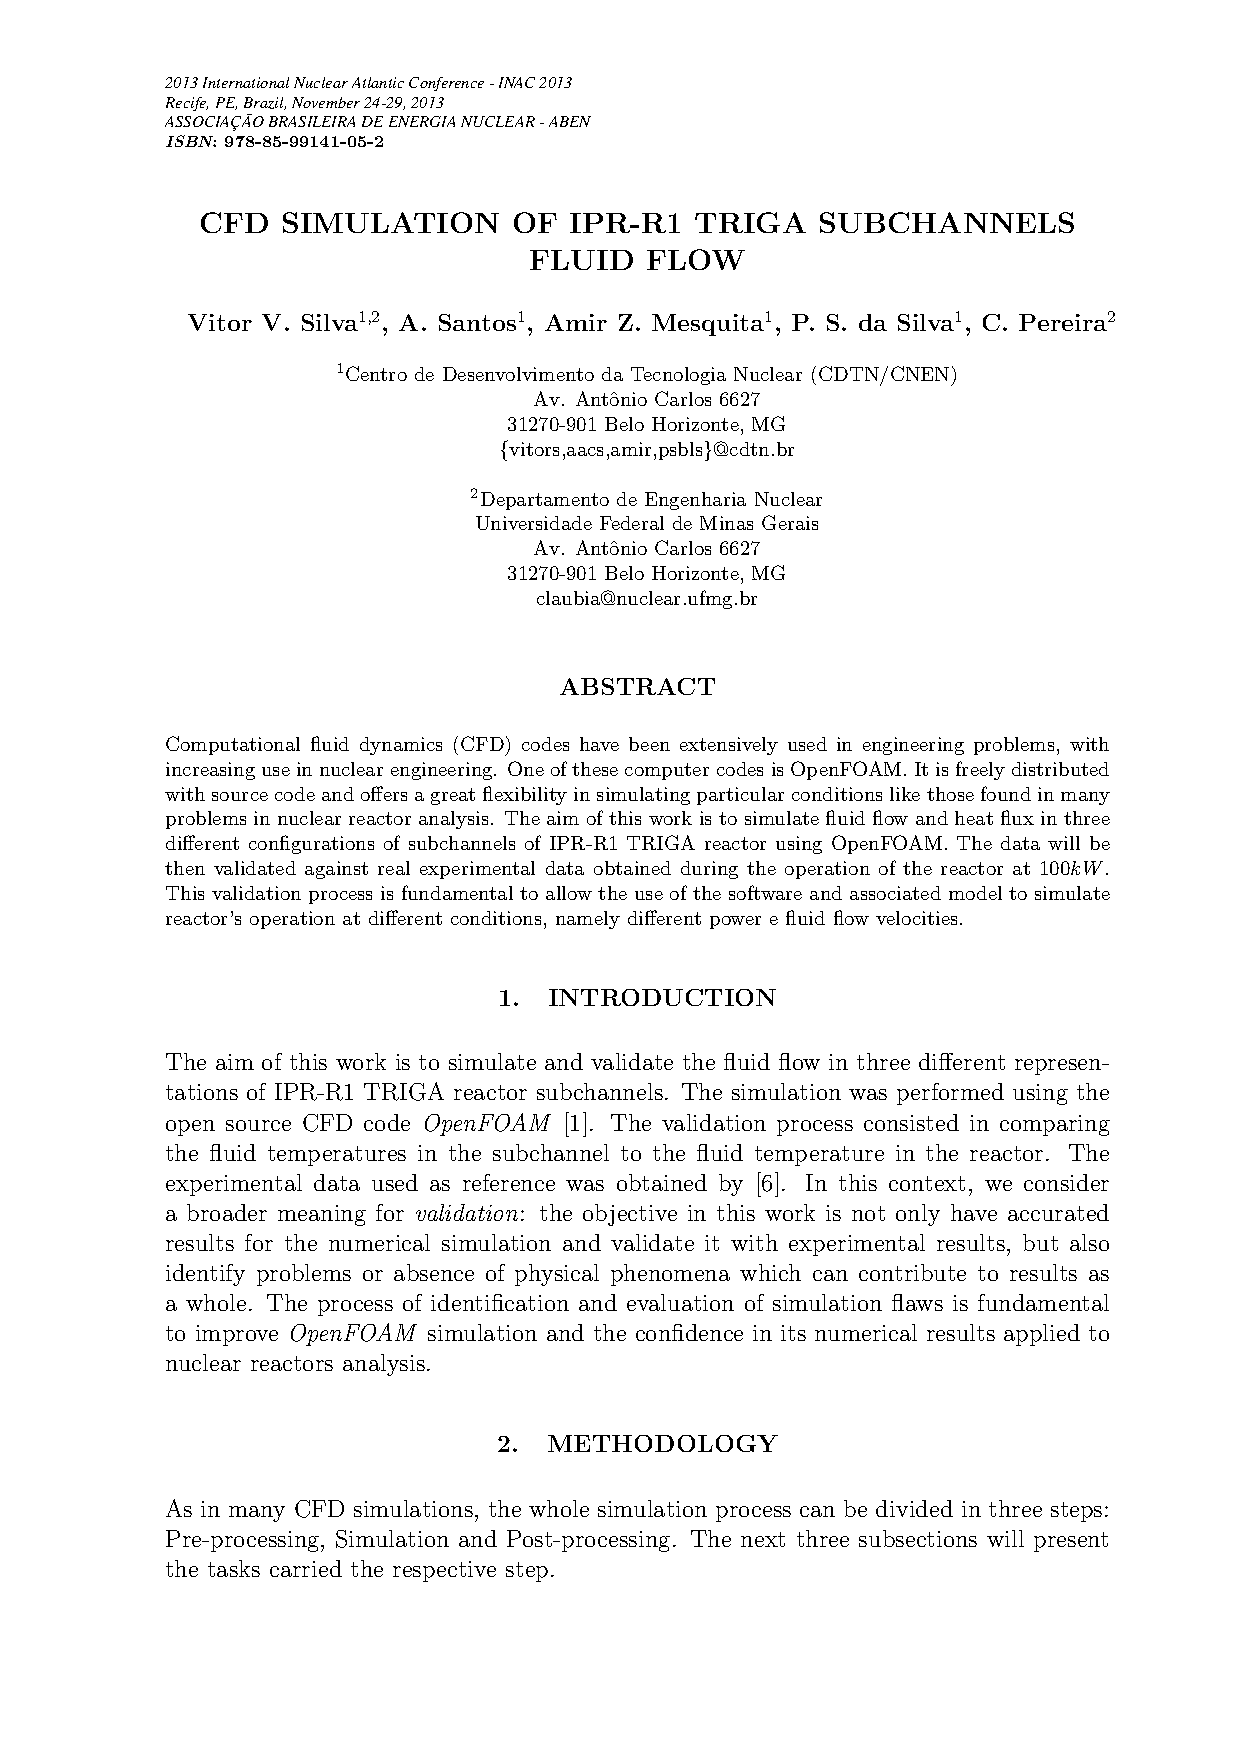
\includepdf[pages={-}]{anexos/inac2013.pdf}

%\chapter{Simulação do combustível do reator TRIGA IPR-R1 com 
%ANSYS/CFX}
%\label{ane:simfuel}


%\chapter{Paper RRFM 2013}
%\label{ane:RRFM2013}
%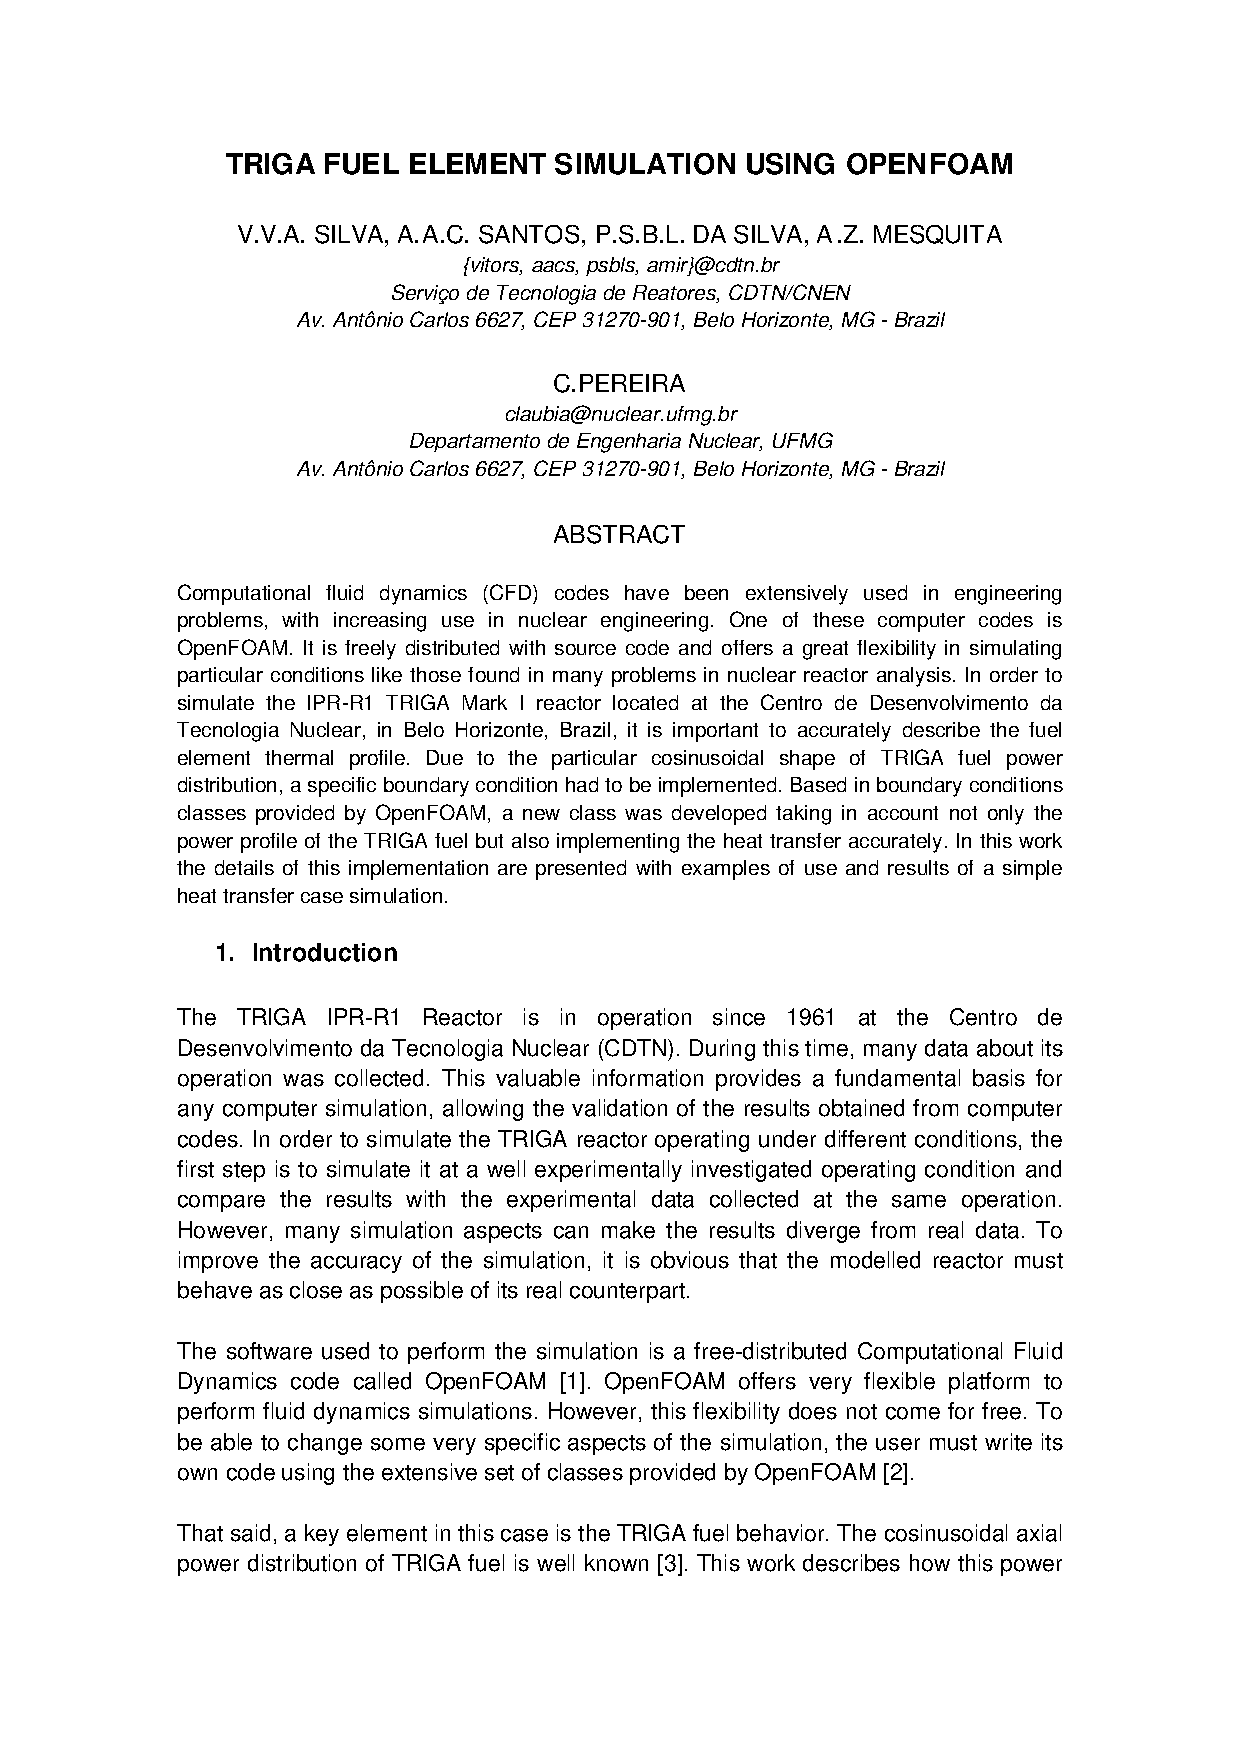
\includepdf[pages={-}]{anexos/RRFM2013}


%\chapter{Pedido do registro de Produto Tecnológico INPI}
%\label{ane:trigafuel}
%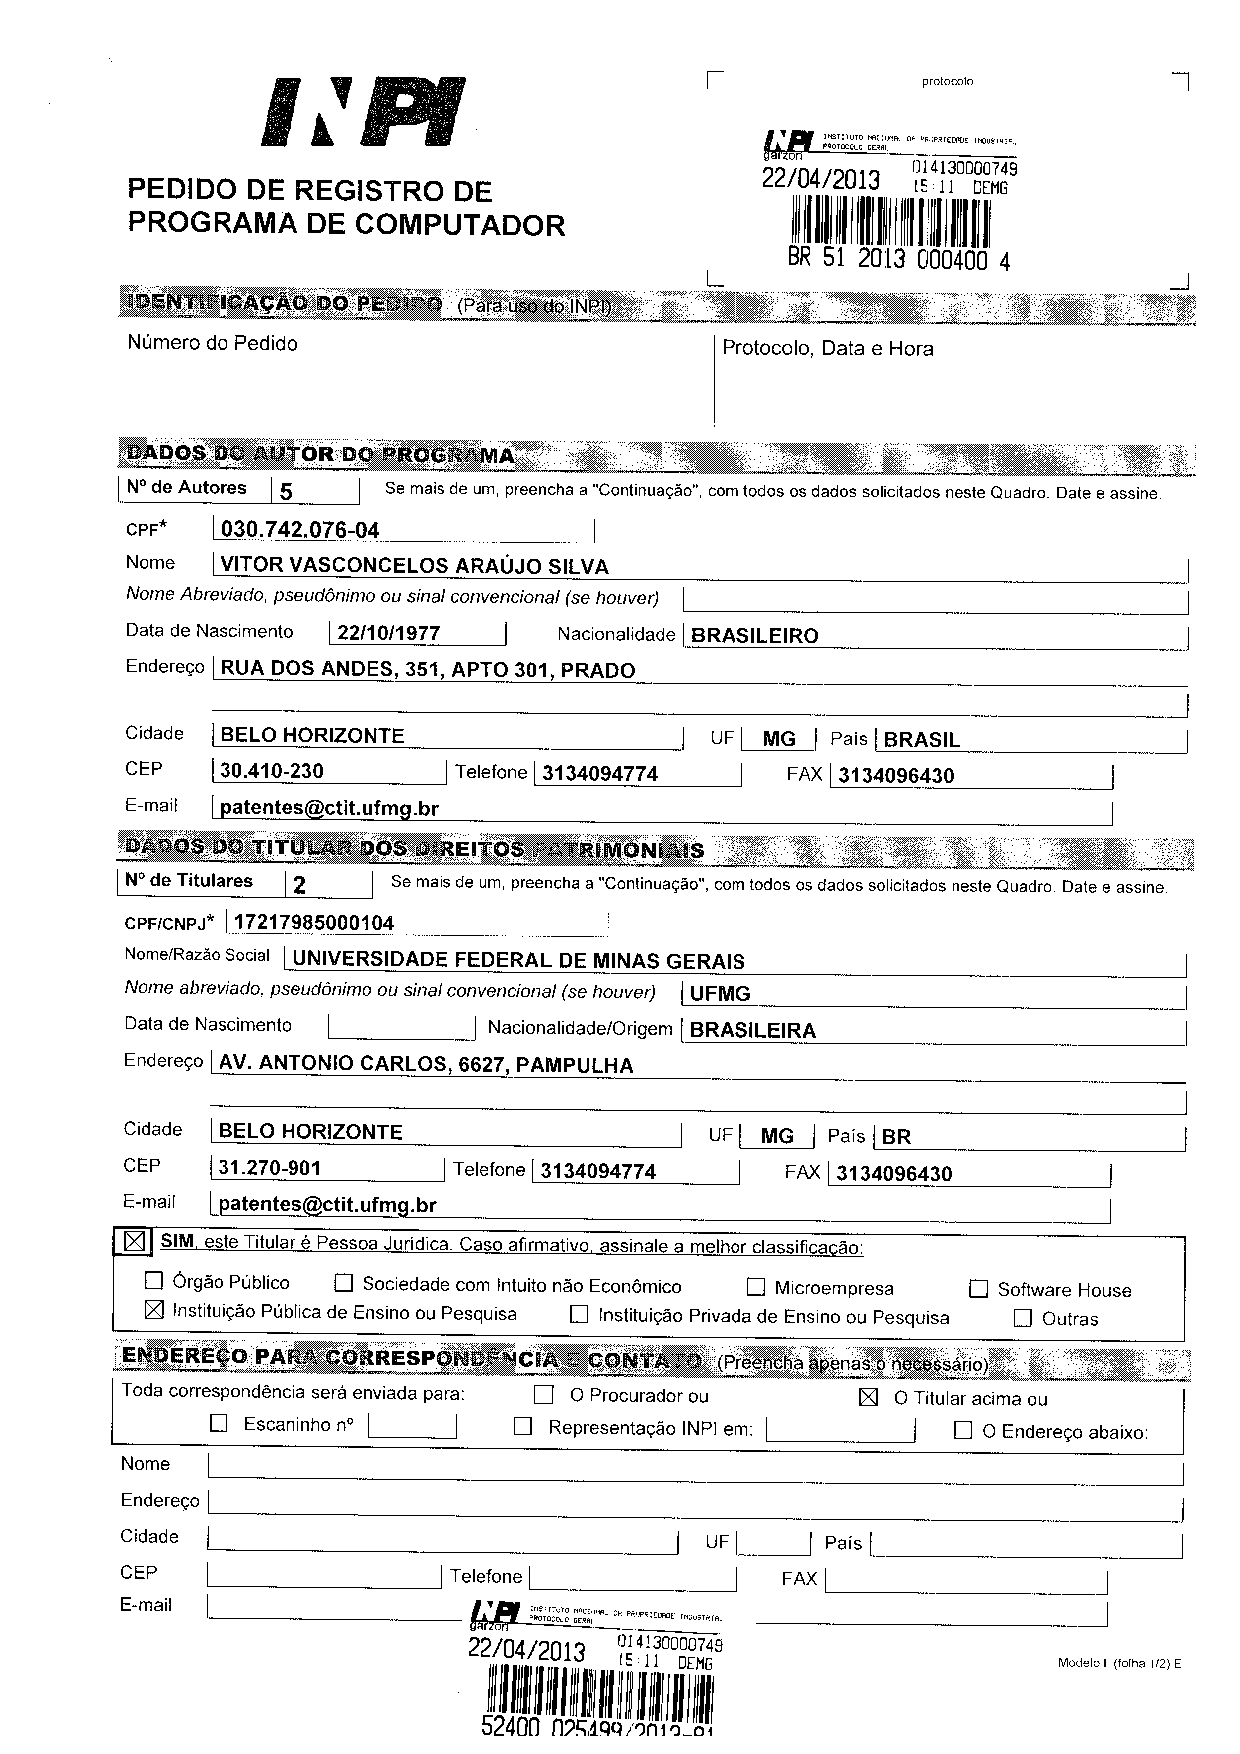
\includepdf[pages={-}]{anexos/depositotrigafuel.pdf}

%\end{anexosenv}

%---------------------------------------------------------------------
% INDICE REMISSIVO
%---------------------------------------------------------------------

\printindex

\end{document}
